% --
% Experiments on whole dataset

\section{Experiments on the whole Dataset}\label{sec:exp_final}
The final experiments were performed on the whole dataset with 3500 examples per labels and are therefore used for comparison to the benchmark models listed in \rsec{prev_kws_benchmark}.
All CNN architectures were evaluated with 12 MFCC coefficients and the application of either frame-based normalization or no normalization.
A single run with 2000 epochs was performed for all experiments to save computational effort.
The evaluation on the adversarial pre-training, as described in \rsec{exp_adv}, was done for the \texttt{conv-jim} model in a separate run.
\rtab{exp_final_l12} shows the results of the experiments.
\begin{table}[ht!]
\small
\begin{center}
\caption{Experiment on the whole dataset with 3500 examples per label, 12 MFCC coefficients and 2000 epochs.}
\begin{tabular}{ M{3cm}  M{1.5cm}  M{2.5cm}  M{2.5cm}  M{2.5cm} }
\toprule
\multirow{2}{*}{\centering\textbf{Model Name}} & \multirow{2}{*}{\centering\textbf{Norm.}} & \multirow{2}{*}{\centering\textbf{Pre-Train}} & \multicolumn{2}{c}{\textbf{Accuracy}}\\
& & & Test set & My dataset\\
\midrule
conv-trad & 0 & - & $84.52$ & $92.00$ \\
conv-fstride & 0 & - & $79.76$ & $80.00$ \\
conv-jim & 0 & - & $87.14$ & $88.00$ \\
\midrule
conv-trad & 1 & - & $83.79$ & $88.00$ \\
conv-fstride & 1 & - & $78.71$ & $92.00$ \\
conv-jim & 1 & - & $82.36$ & $88.00$ \\
\midrule
conv-jim & 1 & adv-label-100 & $84.62$ & $92.00$ \\
\bottomrule
\label{tab:exp_final_l12}
\end{tabular}
\end{center}
\vspace{-4mm}
\end{table}
\FloatBarrier
\noindent
Note that there are some overfitting effects happening, especially showing up in the not normalized training of the \texttt{conv-trad} model in \rfig{exp_final_loss_conv-trad}.
It is therefore useful to apply an early stopping technique for better generalization, that obtains the model parameters at the best performing training epoch evaluated on the validation set.
\begin{figure}[!ht]
  \centering
  \subfigure[norm0]{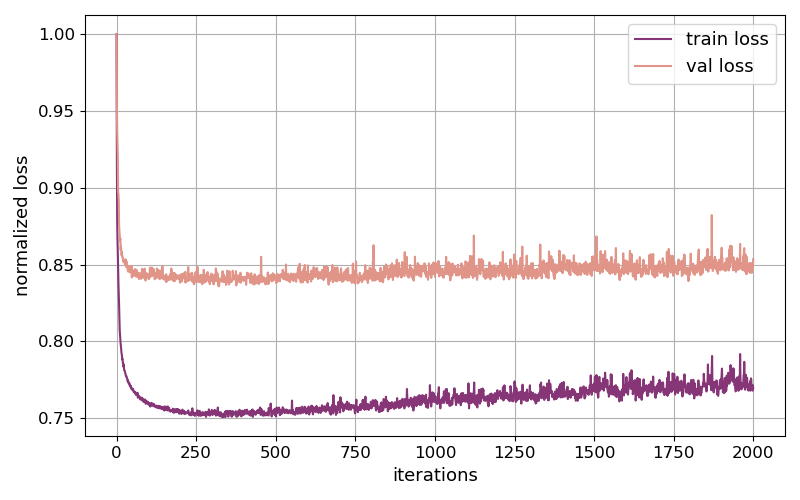
\includegraphics[width=0.45\textwidth]{./5_exp/figs/exp_final_loss_norm0_conv-trad.png}}
  \subfigure[norm1]{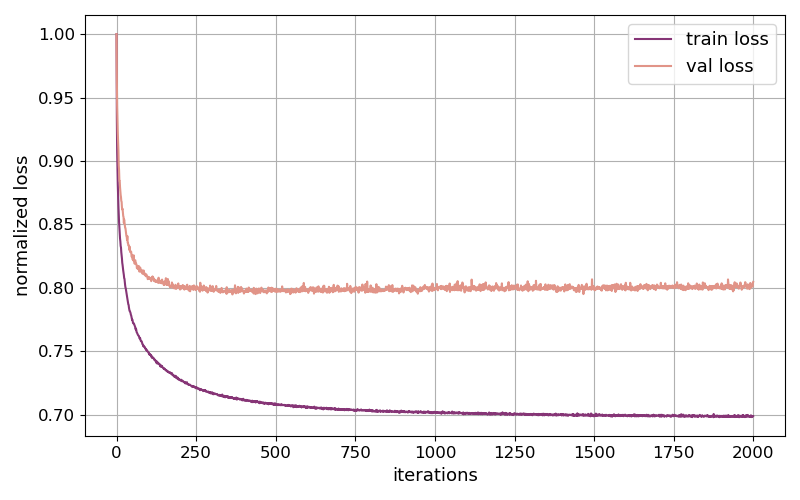
\includegraphics[width=0.45\textwidth]{./5_exp/figs/exp_final_loss_norm1_conv-trad.png}}
  \caption{Training loss of the \texttt{conv-trad} model showing overfitting effects on the whole dataset.}
  \label{fig:exp_final_loss_conv-trad}
\end{figure}
\FloatBarrier
\noindent
The training of models with frame-based normalization has usually fewer problems with overfitting compared to the case when no normalization was applied.
The accuracy performance on the validation set of all models with and without frame-based normalization is shown in \rfig{exp_final_acc}.
\begin{figure}[!ht]
  \centering
  \subfigure[norm0]{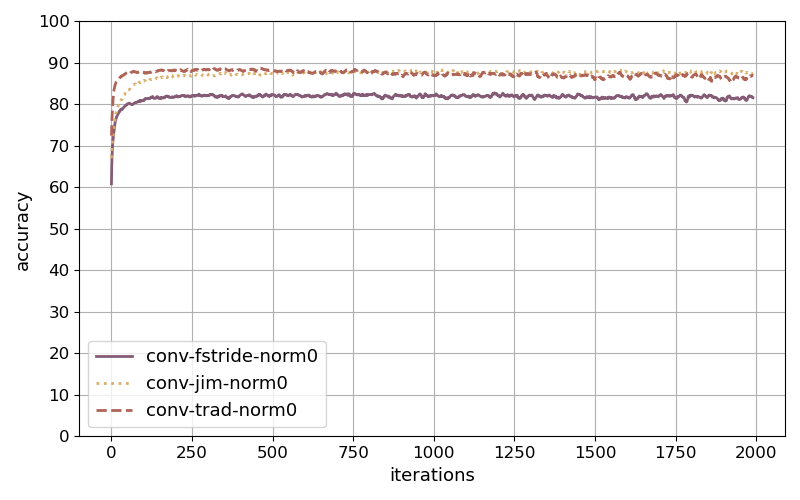
\includegraphics[width=0.45\textwidth]{./5_exp/figs/exp_final_acc_norm0.png}}
  \subfigure[norm1]{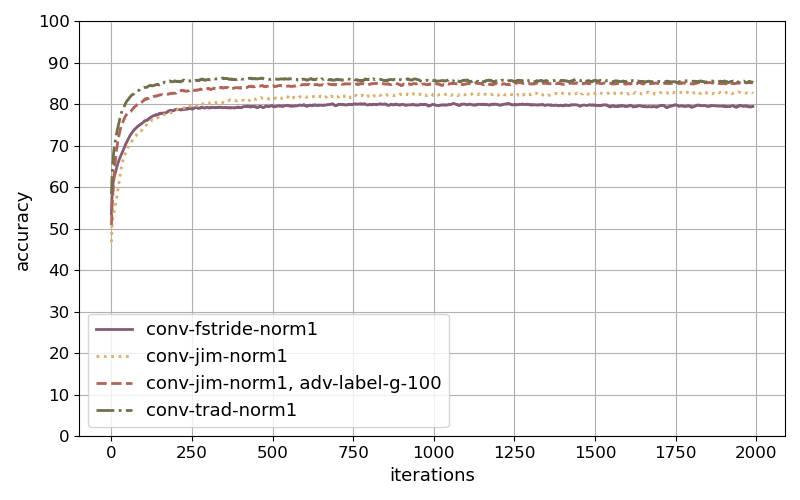
\includegraphics[width=0.45\textwidth]{./5_exp/figs/exp_final_acc_norm1.png}}
  \caption{Training accuracies of all models with and without frame-based normalization performed on the whole dataset, averaged over 10 epochs for better visualization.}
  \label{fig:exp_final_acc}
\end{figure}
\FloatBarrier
\noindent
Note that the accuracy scores had been smoothed over the epochs and that usually some spikes in performances are present and should be avoided.
Therefore, it is strongly recommended to use early stopping.
For instance, the \texttt{conv-trad} without frame-based normalization could have got a better score if early stopping would have been used.

There is a large gap between the evaluated models and the benchmark models in \rsec{prev_kws_benchmark}.
With \SI{84.62}{\percent} the \texttt{conv-jim} model with adversarial pre-training performs about \SI{10}{\percent} worse than the benchmark model (DS-CNN-S \cite{Zhang2017}) with \SI{94.4}{\percent}.
Although it has to be considered that the amount of operations for the \texttt{conv-jim} model are about 6 times lower than the DS-CNN-S and that not the whole audio file of \SI{1}{\second} was processed but a shorter time interval of \SI{500}{\milli\second}.
With this in mind, the results do not look that poor.
To observe the problems in classification, a confusion matrix from the \texttt{conv-jim} model with adversarial label train on the Generator weights, is shown in \rfig{exp_final_confusion}.
\begin{figure}[!ht]
  \centering
  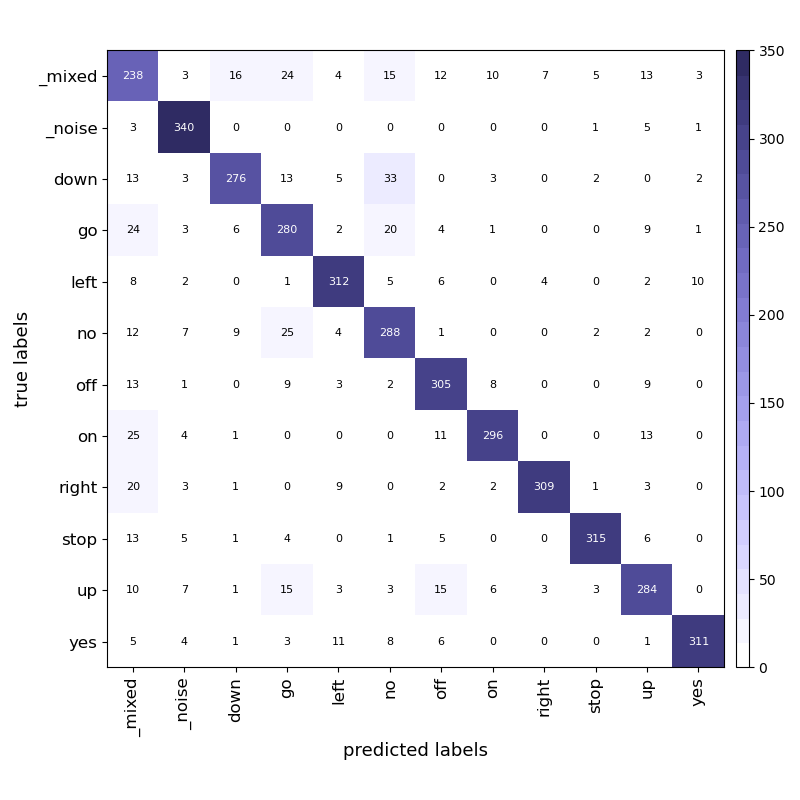
\includegraphics[width=0.45\textwidth]{./5_exp/figs/exp_final_confusion.png}
  \caption{Confusion matrix of the \texttt{conv-jim} model pre-trained with adversarial label train of 100 epochs using the Generator weights and 2000 training epochs applied with frame-based normalization.}
  \label{fig:exp_final_confusion}
\end{figure}
\FloatBarrier
\noindent
From the confusion matrix, it can be observed that most classifications were correct and misconceptions usually happened at similar words with the same phoneme structure like \enquote{go} and \enquote{no}.
The mixed labels also added more difficulty to the KWS task and decreased the overall classification performance.

\rsec{appendix_weights} visualizes the weights of the first convolutional layers of the trained models.
All in all, the obtained scores should be sufficient for a video game application.